\chapter{Diseño e implementación} % Main chapter title

\label{Chapter3} % Change X to a consecutive number; for referencing this chapter elsewhere, use \ref{ChapterX}

\definecolor{mygreen}{rgb}{0,0.6,0}
\definecolor{mygray}{rgb}{0.5,0.5,0.5}
\definecolor{mymauve}{rgb}{0.58,0,0.82}

%%%%%%%%%%%%%%%%%%%%%%%%%%%%%%%%%%%%%%%%%%%%%%%%%%%%%%%%%%%%%%%%%%%%%%%%%%%%%
% parámetros para configurar el formato del código en los entornos lstlisting
%%%%%%%%%%%%%%%%%%%%%%%%%%%%%%%%%%%%%%%%%%%%%%%%%%%%%%%%%%%%%%%%%%%%%%%%%%%%%
\lstset{ %
  backgroundcolor=\color{white},   % choose the background color; you must add \usepackage{color} or \usepackage{xcolor}
  basicstyle=\footnotesize,        % the size of the fonts that are used for the code
  breakatwhitespace=false,         % sets if automatic breaks should only happen at whitespace
  breaklines=true,                 % sets automatic line breaking
  captionpos=b,                    % sets the caption-position to bottom
  commentstyle=\color{mygreen},    % comment style
  deletekeywords={...},            % if you want to delete keywords from the given language
  %escapeinside={\%*}{*)},          % if you want to add LaTeX within your code
  %extendedchars=true,              % lets you use non-ASCII characters; for 8-bits encodings only, does not work with UTF-8
  %frame=single,	                % adds a frame around the code
  keepspaces=true,                 % keeps spaces in text, useful for keeping indentation of code (possibly needs columns=flexible)
  keywordstyle=\color{blue},       % keyword style
  language=[ANSI]C,                % the language of the code
  %otherkeywords={*,...},           % if you want to add more keywords to the set
  numbers=left,                    % where to put the line-numbers; possible values are (none, left, right)
  numbersep=5pt,                   % how far the line-numbers are from the code
  numberstyle=\tiny\color{mygray}, % the style that is used for the line-numbers
  rulecolor=\color{black},         % if not set, the frame-color may be changed on line-breaks within not-black text (e.g. comments (green here))
  showspaces=false,                % show spaces everywhere adding particular underscores; it overrides 'showstringspaces'
  showstringspaces=false,          % underline spaces within strings only
  showtabs=false,                  % show tabs within strings adding particular underscores
  stepnumber=1,                    % the step between two line-numbers. If it's 1, each line will be numbered
  stringstyle=\color{mymauve},     % string literal style
  tabsize=2,	                   % sets default tabsize to 2 spaces
  title=\lstname,                  % show the filename of files included with \lstinputlisting; also try caption instead of title
  morecomment=[s]{/*}{*/}
}


%----------------------------------------------------------------------------------------
%	SECTION 1
%----------------------------------------------------------------------------------------
En este capítulo se detallan los aspectos técnicos del desarrollo del trabajo. Incluye las consideraciones tomadas en cuenta durante el desarrollo, el detalle de las modificaciones realizadas al modelo de partida, así como el detalle del papel que juega el módulo en el sistema. De igual manera, se hace una descripción cronológica del desarrollo del módulo.    

\section{Consideraciones generales}

El módulo de inteligencia artificial propuesto es una implementación del modelo YOLOv3, especialmente modificada para cumplir con las necesidades específicas del cliente, así como una serie de requisitos funcionales.  Es por esto que fue necesario hacer modificaciones a los archivos originales de la biblioteca. 

Como se puede observar en el capítulo 1, no todos los requerimientos funcionales propuestos para el inicio del trabajo pudieron ser cubiertos. Recordando que esta versión del trabajo representa un mínimo producto viable, a continuación se presenta una lista de todos los requerimientos funcionales que fueron cubiertos:

\begin{itemize}

	\item El módulo se ejecuta en un computador de uso de hogar. 
	\item El módulo es capaz de reconocer 14 clases como intruso. 
	\item Se reporta al usuario de manera visual. 
	\item Se reporta al usuario a través de un archivo de fácil análisis.
	\item Resulta muy sencillo iniciar la ejecución del módulo a través de su interfaz grafica. 

\end{itemize}

De igual manera, el módulo está construido de manera que realizar modificaciones, o bien, expandir su funcionalidad en un futuro resulte muy sencillo. Es de vital importancia recalcar que esto se hizo teniendo en cuenta que se trata de un módulo que, a fin de salir de este estatus de mínimo producto viable, deberá sufrir un proceso de optimizacion muy fuerte. Algunos ejemplos de puntos en los que se pueden aplicar estos trabajos son:

\begin{itemize}

	\item El módulo está diseñado para filtrar las etiquetas que no hacen parte de las clases dadas en la definición de intruso. Esto implica que, a pesar de que no se reporte en ninguna de las dos metodologías, el módulo aún reconoce otras clases. En otras palabras, si se puede observar un modelo en el \textit{frame}, este será satisfactoriamente detectado y son los métodos encargados del reporte los que no lo entregarán como un resultado positivo. 
	\item La precisión del modelo debe ser mejorada: dado que ocasionalmente se hacen detecciones de objetos que no corresponden con lo visto en el \textit{frame}. Se detectó que, en particular, el módulo es especialmente susceptible a generar falsos positivos. 
	\item Los cuadros se devuelven en espacio de color bgr. Esto, en combinación con que el color de los rectángulos no se puede cambiar desde la interfaz grafica.
	\item El color de los rectángulos es igual para todas las clases de objeto.
	\item Se debe mejorar significativamente el manejo que da el módulo de las excepciones que se generen, tanto a nivel de manejo de problemas originados en el código mismo, como recuperación cuando se generen cortes en la recepcion del \textit{streaming} de video.
	\item A pesar de que la interfaz grafica se realizó pensando en la facilidad de uso para el usuario, su comportamiento podría resultar extraño dado que el diseño de experiencia de usuario (UX) quedó fuera del alcance de los trabajos durante su etapa de concepción. 

\end{itemize}

Finalmente, resulta de especial interés tener en mente también las limitaciones del modelo:

\begin{itemize}

	\item Los modelos YOLO se ven limitados cuando se les pide detectar objetos que se encuentran muy cerca de una fuente de luz muy brillante, especialmente el sol, se pueden generar dificultades para detectar los objetos. Esto es parcialmente contrarrestado añadiendo las clases adicionales detalladas en la tabla \ref{clases-auxiliares-etiquetas}. 
	\item Los objetos deben encontrarse a una distancia prudencial del dron. A pesar de que las pruebas de vuelo no se han enfocado en el cálculo de este valor, sí se hace evidente que al estar el dron demasiado lejos de ellas, no se hace una detección oportuna. 
	\item El modelo no cuenta con funciones de \textit{auto-healing}, que deberían ser tenidas en cuenta a fin de lograr mantener la integridad del modelo si sus pesos son actualizados constantemente por el cliente a fin de mejorar la predicción. 

\end{itemize}

\section{Arquitectura del módulo}

Se propone como mínimo producto viable de este módulo, un código altamente modular. Esto significa que la manera en la que está desarrollado (a excepción del método principal, en el archivo Utils), está planteada en pequeños métodos que podrán ser modificados y mantenidos con facilidad. Esto supone, sin embargo, que sea de vital importancia entender la arquitectura del módulo a fin de poder realizar las modificaciones pertinentes en el punto adecuado del código. Así como se hizo en el numeral anterior (consideraciones generales) con el flujo de información entre el sistema y el módulo, a continuación, se describe el flujo de la información en el interior del módulo.   

El módulo está compuesto por cuatro capas funcionales:

\begin{enumerate}

	\item Funciones originales de YOLO: encargadas de la funcionalidad base de detección de los objetos en la totalidad de las clases que componen el \textit{dataset} COCO. Incluye funciones como nms (encargada del \textit{non-max supression}) y la función IoU. 
	\item Funciones híbridas: normalmente funciones que coordinan el llamado de las demás funciones. A pesar de que ofrecen una funcionalidad muy similar a las originales de YOLO, funcionan en un orden diferente, de forma que se puedan obtener los datos requeridos en el momento preciso para las necesidades del cliente.  
	\item Funciones propias: que permiten agregar al módulo la funcionalidad requerida por el cliente. Ejemplos de estas funciones incluyen la generación de archivos en formato CSV y la carga de etiquetas válidas. 
	\item Interfaz gráfica: que permite al usuario interactuar con el módulo para iniciar su ejecución fácilmente. 

\end{enumerate}

El diagrama de bloques correspondiente a estas cuatro capas es el siguiente:

\begin{figure}[!ht]
    \centering
    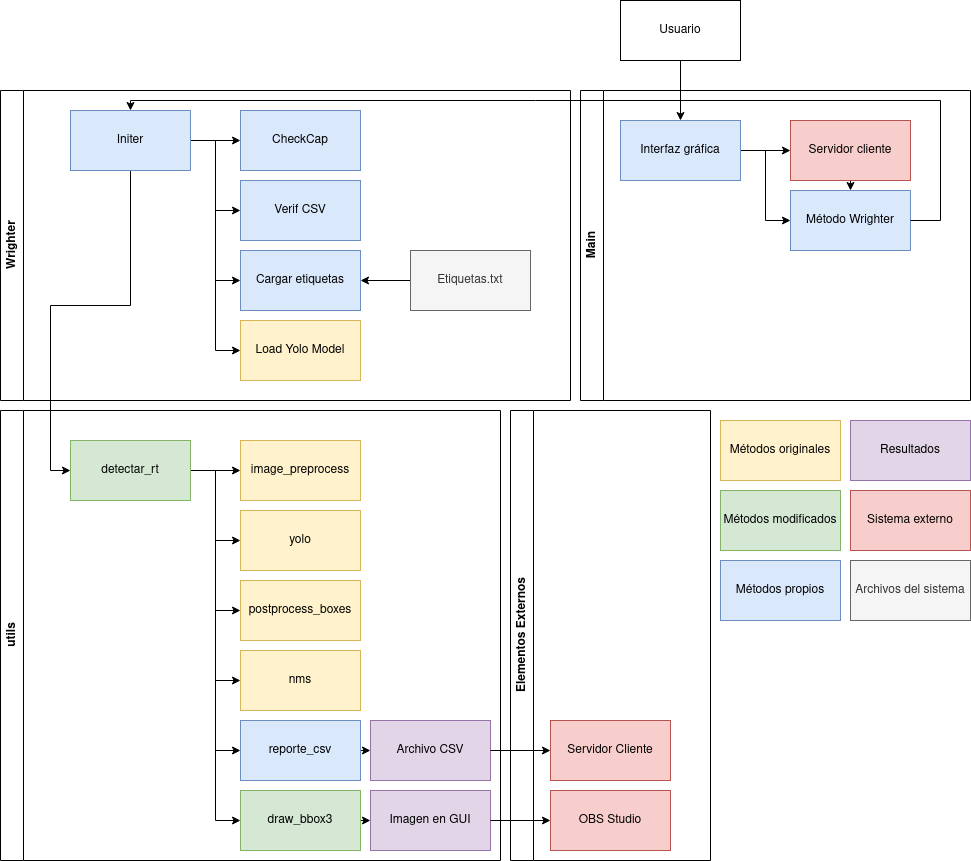
\includegraphics[width=16cm, height=14cm]{c31v2}
    \caption{Diagrama de bloques del módulo.}
    \label{fig:mesh1}
\end{figure}


\section{Esquema detallado del módulo en el interior del sistema}

Este módulo es una parte de un trabajo más grande desarrollado directamente por el cliente. Es decir, deberá estar en capacidad de comunicarse con otras partes del sistema, de forma que estos otros módulos puedan tomar decisiones y recibir órdenes de controladores humanos. A pesar de que se desconoce el funcionamiento de la totalidad del sistema.  

Para lograr esto, durante la fase de concepción del trabajo se estipuló que el módulo deberá ser capaz de conectarse a los servidores del cliente, en los que se aloja la transmisión de vídeo. Esta conexión entre ambos equipos se logra cuando el usuario indica al módulo, a través de la interfaz gráfica (visible en la imagen). Una vez se presiona el botón “Iniciar ejecución”. Esta interfaz está pensada para ser tan sencilla como sea posible, permitiendo que el usuario inicie la ejecución del módulo de la manera más sencilla posible.

\begin{figure}[!ht]
    \centering
    
\includegraphics[width=10cm, height=2cm]{c32}
    \caption{Interfaz gráfica del módulo.}
    \label{fig:gui}
\end{figure} 

Por otro lado, el módulo deberá reportar al resto del sistema si se detectó a algún intruso. Para esto, se definieron dos metodologías, que se detallarán más adelante en este capítulo:

\begin{enumerate}

	\item Reporte visual
	\item Reporte en formato CSV

\end{enumerate}

Dada esta descripción, desde afuera, el módulo tendrá el siguiente aspecto:

\begin{figure}[!ht]
    \centering
    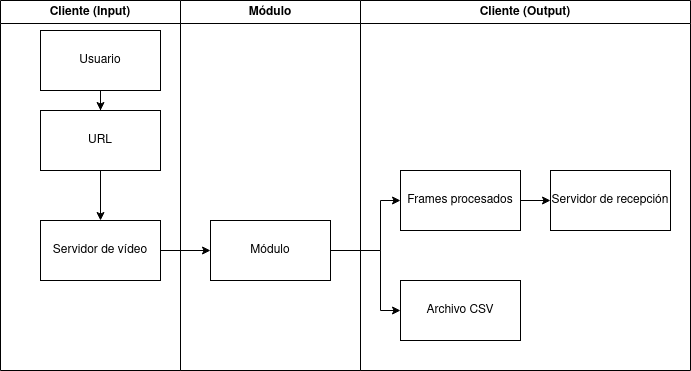
\includegraphics[width=16cm, height=9cm]{c33v2}
    \caption{Diagrama de bloques del módulo en el interior del sistema.}
    \label{fig:mesh1}
\end{figure} 

Cabe mencionar que, dada la naturaleza confidencial de este módulo, así como de la totalidad del sistema, se buscó que el módulo requiriera la menor cantidad de información para funcionar como fuese posible. Esto también permite que los parámetros dados del vídeo y la cantidad de transmisiones que se procesan a la vez se encuentren bajo total control del cliente. 

De igual manera es de vital importancia tener en cuenta que la totalidad del módulo se desarrolló sin conocer el funcionamiento del resto del sistema. Es por esto que para iniciar su ejecución se debe ejecutar el código de manera manual. El sistema no puede detectar cuándo se ha iniciado una transmisión, y por lo tanto, se requiere de una persona encargada de dar inicio cuando sea necesario. 

Finalmente, este módulo está diseñado como un mínimo producto viable que permita a las personas tomar decisiones informadas, con soporte en vídeo. Esta versión no se considera un sistema autónomo, sino que constituye un sistema de apoyo a la decisión. 


\section{Esquema detallado de las modificaciones hechas al modelo}

Dado que se trata de una implementación personalizada, existen varias diferencias entre el módulo desarrollado y la implementación original del modelo YOLOv3. Dicho esto, las modificaciones realizadas generales al modelo, en orden cronológico son las siguientes:

\begin{itemize}

	\item Se preparó el código para que se ejecute desde un \textit{streaming} de vídeo, en vez de un archivo local en el equipo. Esto implica que se debe detener la ejecución antes de pasar imágenes al método de detección si no es posible establecer conexión con el servidor.
	\item Se filtraron las etiquetas a fin de lograr que solo sean detectadas las clases definidas en la definición de intruso.
	\item Se crearon los métodos encargados de generar una respuesta que se pasará al resto del módulo. Particularmente, se le permitió al programa generar dos tipos de respuesta.
	\item Se estableció un método que permite descartar un número determinado de \textit{frames}, de forma que se permita aliviar la carga computacional sobre el equipo.
	\item Durante el desarrollo del módulo se estableció que el hacer que el módulo sea capaz de procesar varios \textit{streamings} de vídeo de manera paralela está fuera del alcance de las temáticas cubiertas en el postgrado, a fin de cubrir satisfactoriamente este requisito, se informó al cliente que sería posible este análisis en caso de que se reciba el \textit{streaming} con varias cámaras combinadas en un único cuadro. Esto, por ser una decisión relacionada con la forma en la que el cliente maneja su \textit{streaming}, no afectó el desarrollo del trabajo. 

\end{itemize}

Cabe resaltar que cada una de estas modificaciones implicó una serie de tareas más pequeñas, a las que Manta Beach, como cliente, hizo un seguimiento cercano.

\section{Ajustes para cumplir con el rendimiento requerido}

Dadas las limitantes del equipo en el que se realizó el desarrollo del módulo (especialmente teniendo en cuenta que este desarrollo se hizo utilizando máquinas virtuales), fue necesario llevar a cabo un análisis detallado que, en teniendo en mente las necesidades del cliente, permitiera reducir la carga computacional sobre la máquina. De esta manera se intentó una serie de ajustes al modelo de forma que se lograra mantener los requisitos dados en el proceso de establecimiento de los trabajos:

\begin{itemize}
 	\item Eliminación de un número determinado de \textit{frames}. Si bien, este es un número fácil de establecer, y que el sistema recibirá como parámetro, se recomienda utilizar un valor de N=10, de forma que, para un fps de 30, se analicen 3 cuadros por segundo. Cabe resaltar que 30 será el número máximo para cumplir con el requisito de hacer un análisis en un tiempo no mayor a 1 segundo, mientras que con N=120, se cumplirá el requisito de hacer un análisis en un tiempo no mayor a 4 segundos.
 	\item Reducción de la calidad del \textit{streaming} de vídeo a 200. A pesar de que esta reducción afecta muy notoriamente la calidad del vídeo, el módulo es capaz de detectar objetos. Se pierden, sin embargo, las propiedades probatorias del trabajo. En la imagen se puede ver un ejemplo del vídeo con calidad reducida. Como se mencionó en secciones anteriores este es un parámetro qué el módulo ya recibe en el \textit{streaming} de vídeo, y cuyo control recae únicamente en el cliente. 
 
\end{itemize}

Finalmente, la solución escogida fue descartar uno de cada N \textit{frames}, de forma que no se procese la totalidad de ellos, y se requiera una mejor cantidad de operaciones. Cabe mencionar que, en este tipo de modelos, es común que conforme se aumente el rendimiento, también se reducirá la precisión del modelo. Es por esto que, para contrarrestar estos efectos, se decidió incluir algunas clases que permitieran hacer una detección indirecta. Estas clases corresponden a objetos que las personas cargan con frecuencia. Estas clases adicionales son: 

\begin{table}[h]
\centering
\caption{Clases auxiliares para detección indirecta.}
\label{clases-auxiliares-etiquetas}
\begin{tabular}{cc}
\hline
\multicolumn{2}{c}{\textbf{Clases auxiliares}} \\ \hline
Camión                	  & Bicicleta              \\
Automóvil                 & Bus		               \\
Motocicleta               & Sombrilla              \\
Mochila			          & Maletín                \\  \hline
\end{tabular}
\end{table}

Por la naturaleza del trabajo, cabe aclarar, en este punto, que el módulo no podrá discernir que al detectar simultáneamente la clase mochila y la clase persona en un espacio muy cercano, podrá tratarse de una única detección. Estas serán registradas y reportadas por el módulo como dos detecciones separadas. 

Esto, sin embargo, es preferible a eliminar detecciones, teniendo en mente que se prefiere que el módulo pueda detectar a tantas personas como sea posible, dada la sensibilidad de las consecuencias en caso de una falla del modelo. 

\section{Entrega de resultados obtenidos al resto del software y retransmisión del vídeo procesado}

Una vez que se ha analizado el \textit{frame}, el módulo deberá ser capaz de devolver resultados al resto del sistema, de forma que tanto las personas encargadas, como el sistema mismo sean capaces de tomar decisiones rápidas, e informar cómo proceder. Dados estos dos actores a los que se les debe hacer llegar la información, en conjunto con el cliente se decidieron utilizar dos métodos diferentes a través de los que el módulo dará su respuesta para cada uno de los \textit{frames}:

\begin{itemize}

	\item Entrega visual: imagen procesada con sus cajas identificando los objetos detectados. Estos \textit{frames} ya procesados son retransmitidos al servidor original para su visualización en la plataforma designada por el cliente. Es importante tener en cuenta que, en esta versión del módulo, esta retransmisión no se hace directamente a través del módulo propuesto, sino que se requerirá el uso de software externo, como el OBS Studio. 
	\item Entrega para análisis de datos: archivo en formato CSV con la información de los objetos detectados. De igual manera, el sistema será capaz de reportar el número del dron desde el que se hizo la detección, a pesar de que es una característica que no se ha probado, teniendo en cuenta que aún no se han hecho vuelos con varios drones de manera simultánea. A diferencia de la imagen preprocesada, este archivo no es retransmitido. Se guarda por defecto en la carpeta de documentos de la máquina en la que se está ejecutando. Visto que esta versión corresponde a un mínimo producto viable, este archivo no se retransmite. Se guarda, en cambio, en la carpeta de documentos de la máquina en la que se ejecuta el módulo. 

\end{itemize}

Es muy importante tener en mente que se espera que no haya personas supervisando constantemente las cámaras. Por este motivo, es posible deshabilitar la retransmisión del \textit{frame} procesado. Por otro lado, y buscando que el sistema sea tan autónomo como resulte posible, no se podrá desactivar el reporte a través de archivos CSV.

\begin{figure}[!ht]
    \centering
    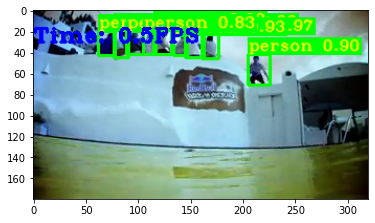
\includegraphics[width=8cm, height=5cm]{sampleGrecia}
    \caption{Ejemplo de resultados generados por el módulo.}
    \label{fig:grecia}
\end{figure}



Por otro lado, los archivos CSV deberán contener los siguientes datos:

\begin{itemize}
	\item Fecha y hora de detección.
	\item Coordenadas de detección dentro del \textit{frame}.
	\item Número de dron en el que ocurre la detección.
\end{itemize}

Los datos serán entregados en el orden en el que han sido mencionados. Esto es de vital importancia de forma que el resto del sistema sea capaz de interpretar correctamente los datos entregados. Por otro lado, se debe recordar que el sistema desconoce la ubicación del dron en su recorrido de vuelo. Es por esto que el módulo no podrá reportar la ubicación en la que detectó el objeto. Esta deberá ser calculada por el sistema a partir de los datos de posición, altura y posición en el \textit{frame} (información proporcionada por el módulo).